\begin{figure}[ht]
\centering
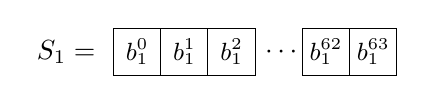
\begin{tikzpicture}

\def\boxw{0.6} % largeur exacte de la boîte
\def\step{\boxw} % PAS = largeur => boîtes collées

% left boxes
\foreach \i/\label in {0/0, 1/1, 2/2} {
    \draw (\i*\step, 0) rectangle (\i*\step+\boxw, 0.6);
    \node[font=\small] at (\i*\step+0.3, 0.3) {$b_1^\label$};
}

% ...
\node at (3*\step+0.33, 0.3) {$\cdots$};

% right boxes
\foreach \i/\clabel in {0/62, 1/63} {
    \draw (4*\step + \i*\step, 0)
        rectangle (4*\step + \i*\step+\boxw, 0.6);
    \node[font=\small] at (4*\step + \i*\step+0.3, 0.3)
        {$b_1^{\clabel}$};
}
% left label
\node at (-0.6, 0.3) {$S_1=$};

\end{tikzpicture}
\end{figure}


Scalar spin & $s_i \in \{-1,+1\}$ \\
Scalar bit & $b_i \in \{0,1\}$ \\


Thus, the obtained phase diagram is in excellent agreement with the expected phase diagram, taking into account that we work on finite size lattices.
